\documentclass[11pt]{article}
\usepackage[utf8]{inputenc}
\usepackage[T1]{fontenc}
\usepackage[margin=1in]{geometry}
\usepackage{graphicx,booktabs,amsmath,amssymb,adjustbox,hyperref}
\setlength{\emergencystretch}{3em}
\title{Train--Test Group Exposure and Source Shift in PCB Defect Detection: A Controlled Benchmark Assurance Study}
\author{Can\thanks{Code and data manifests: \url{https://github.com/canblmz1/openinspect-trust}. Affiliation and contact e-mail to be added.}}
\date{}
\begin{document}
\maketitle
\begin{abstract}
Random train/test splits of industrial inspection datasets can place structurally related images on both sides of the split. We measure how much this train--test group exposure inflates a PCB defect-detection benchmark built from three public datasets (4,420 images, four classes), grouped by machine-detected visual similarity (DINOv2, perceptual hashes) and source metadata. Two training sets, identical except that one contains the group-mates of designated probe test images and the other profile-matched replacements, are evaluated on one byte-identical test set; unexposed control images are a negative control (three designs, eight matched YOLO11n seed pairs). The pre-specified primary endpoint, the probe mAP50-95 difference in the first design, was +3.91 points (95\% interval including seed variation: +0.41 to +7.65). Pooled over designs, probes gained +3.70 (+1.71 to +5.70) and probe minus control was +3.37 (+0.68 to +6.06); the whole-test-set effect was about +2 points. Replication was mixed: an anomalous control gain in one design did not recur, the probe-selective pattern vanished in one seed of another, and the first design's probe-minus-control interval includes zero. Gains concentrated in visually linked and in the most strongly exposed probes (+6.85; positive in all eight seed pairs, including three trained after the stratum was defined), but the continuous similarity--gain association was weak. Holding out a source cost 27--47 points; since image size and format identify the source, this reflects acquisition shift. AI-assisted visual adjudication found no near-duplicates among 60 probe--mate pairs; independent human validation was not performed.

\end{abstract}
\section{Introduction}
Benchmark scores are only as trustworthy as the separation between training and evaluation data. In industrial visual inspection, datasets are often assembled from crops of a limited number of boards, scans or production lots. A random split can therefore place images that share a board, a layout or a capture session on both sides of the train/test boundary. The resulting dependency is analogous to subject-level leakage in medical imaging. It may make reported accuracy partly a measure of familiarity with specific boards rather than of defect detection.

The general phenomenon is well documented: near-duplicates in classification benchmarks~\cite{barz2020}, same-object duplicates in licence-plate recognition~\cite{laroca2023}, subject-level leakage in volumetric medical imaging~\cite{tampu2022}, frame-level leakage in video-derived detection datasets~\cite{figueiredo2024}, and similarity-aware splitting tools~\cite{joeres2025datasail}. Distribution shift between acquisition conditions is equally well known in industrial inspection~\cite{zhang2023aebad,pemula2025robustad}. What is less often measured is the \emph{size} of group-exposure optimism under controlled conditions in industrial object detection, and how it compares, in the same study, with the loss incurred when a detector meets an unseen acquisition source.

We ask two questions:

1. When PCB test images have machine-detected group-related images in the training set, is the performance difference concentrated on those exposed test images? 2. How does that effect compare with the performance loss on a held-out source?

We do not claim to have discovered leakage or to introduce a new splitting method. Our contribution is a controlled measurement with these elements:

\begin{itemize}
\item a fixed common test population and a training-set manipulation that differs only in group exposure;
\item a within-test negative control (unexposed control images);
\item three independently drawn designs and eight matched seed pairs;
\item separate reporting of test-sampling and training-seed uncertainty, and permutation (placebo) tests;
\item a pre-defined exposure-strength stratification;
\item a source-held-out comparison within the same study;
\item a reproducible provenance and split-assurance pipeline.
\end{itemize}
We did not identify prior work combining these elements in PCB defect detection. Our literature search was limited (Section 2), so this is a statement about what we found, not a priority claim.

\section{Related Work}
\textbf{Near-duplicate contamination.} Barz and Denzler found that 3.3\% (CIFAR-10) and 10\% (CIFAR-100) of test images have duplicates in the training set and released duplicate-free test sets~\cite{barz2020}. Laroca et al. showed that near-duplicates of the same licence plate across splits bias licence-plate recognition: error rates more than doubled under duplicate-free (``fair'') splits, and model rankings changed~\cite{laroca2023}. Not every audit finds large effects: Sun et al. removed near-duplicates of their pre-training data from COCO minival and reported minimal impact on detection results~\cite{sun2017revisiting}.

\textbf{Group and subject-level leakage.} Tampu et al. showed that slice-level instead of subject-level splitting of OCT volumes inflates classification performance (MCC +0.07 to +0.43; accuracy +5 to +30\%)~\cite{tampu2022}. Figueiredo and Mendes showed that randomly splitting highly correlated frames of video-derived object-detection datasets causes information leakage, and proposed cluster-based splitting evaluated with YOLOv8~\cite{figueiredo2024}. Joeres et al. formulate leakage-reduced splitting as an optimisation problem (DataSAIL)~\cite{joeres2025datasail}. Our setting is the detection analogue of subject-level leakage. The ``subject'' is a machine-detected group rather than a known patient or video ID.

\textbf{Controlled leakage experiments.} Babu et al. deliberately moved increasing fractions of test images into the training set of an automotive object detector and evaluated on the same test set~\cite{babu2024leakage}. Their manipulation injects copies of test images. Ours swaps naturally occurring group-mates for profile-matched replacements and separates exposed from unexposed images within one test set.

\textbf{Source and domain shift in industrial inspection.} AeBAD~\cite{zhang2023aebad} and Robust AD~\cite{pemula2025robustad} document large performance drops of anomaly detectors under acquisition changes (illumination, viewpoint, background). UniPCB aggregates public PCB imagery from multiple modalities into a vision-language benchmark~\cite{sun2026unipcb}. Our source-held-out arm reports the same kind of shift for supervised PCB defect detection. It also shows that source identity is trivially encoded in image metadata.

\textbf{Position of this work.} Leakage, near-duplicate contamination, group-aware splitting and domain shift are all known. This paper is a controlled case study: it measures how much group exposure inflates a specific industrial detection benchmark, how selective that inflation is, and how it compares with source shift.

\emph{Literature-search limitation.} SciSpace and Scite were not available. References were verified against publisher pages, DOIs, arXiv and PubMed/PMC (\texttt{paper/CITATION\_AUDIT.md}), but no systematic citation-context analysis was done.

\section{Datasets and Provenance}
We pool three public PCB defect datasets, all licensed CC BY 4.0, into one release (v0.1; 4,420 images; 5,297 boxes). The release uses a shared four-class taxonomy: short, open, mouse bite, spurious copper.

\begin{table}[htbp]\centering\small
\begin{adjustbox}{max width=\linewidth}
\begin{tabular}{llllll}
\toprule
source & ingested & released images & released boxes & image form & acquisition (as described by the source) \\ \midrule
DsPCBSD+~\cite{lv2024dspcbsd} & 10,259 & 1,768 & 2,472 & 226 px JPG (39 at 108 px) & production PCB images from an industrial manufacturer \\
PCB-IND~\cite{yan2026pcbind} & 4,789 & 1,713 & 1,854 & 300 px JPG & inline industrial AOI system \\
PCB-Defect~\cite{rashid2025pcbdefect} & 230 & 939 crops & 971 & PNG crops, mostly 300 px & high-resolution images of laboratory-fabricated single-layer FR4 boards \\
\bottomrule
\end{tabular}
\end{adjustbox}
\end{table}
\textbf{Selection.} Released images contain only the four benchmark classes. DsPCBSD+ was sampled per class set to keep every source at or below 40\% of the release. PCB-Defect's high-resolution images were cropped around defects (minimum side 300 px, 10\% margin), and crops that cut a box or overlapped another crop were excluded.

\textbf{Provenance.} Every released image keeps its source item, SHA-256 hash and crop parent. Licence evidence, taxonomy mappings, label audits and split manifests are versioned and re-derived in continuous integration. Releasing a modified subset requires indicating the changes, as CC BY requires.

\section{Group Construction}
\textbf{Embeddings and thresholds.} Whole images are embedded with DINOv2-small~\cite{oquab2024dinov2} (primary) and DINOv2-base (sensitivity). Cosine thresholds were fixed by a rule committed before any model was trained:

\begin{itemize}
\item near level: 0.934, the 95\%-recall point on synthetic transformed duplicates;
\item family level: 0.918, the F1-optimal point on metadata-defined pools.
\end{itemize}
A perceptual-hash distance $\leq$ 4 flags review candidates. Each source uses its own primary level (family for DsPCBSD+ and PCB-IND, near for PCB-Defect).

\textbf{Constraint groups.} An image's constraint group is the transitive union of three links:

\begin{itemize}
\item its similarity component;
\item its source metadata group (for PCB-IND, the board identifier in the file name);
\item its crop parent (for PCB-Defect).
\end{itemize}
We call these \emph{machine-detected visual-similarity groups}, not duplicates.

\textbf{Representation sensitivity.} The groups depend on the embedding. Within DsPCBSD+ and PCB-IND, DINOv2-small and DINOv2-base components barely overlap (adjusted Rand index about 0.01). About 43\% of design-0 probes would not be exposed under DINOv2-base constraint groups.

\section{Controlled Experimental Design}
Each design D $\in$ \{D0, D1, D2\} is an independent random draw with identical parameters:

\begin{table}[htbp]\centering\small
\begin{adjustbox}{max width=\linewidth}
\begin{tabular}{llll}
\toprule
 & D0 & D1 & D2 \\ \midrule
test images (probes / controls) & 407 (194 / 213) & 408 (193 / 215) & 409 (194 / 215) \\
validation images & 698 & 699 & 698 \\
training images per condition & 3,102 & 3,099 & 3,103 \\
swapped images (mates $\leftrightarrow$ replacements) & 213 & 214 & 210 \\
\bottomrule
\end{tabular}
\end{adjustbox}
\end{table}
\textbf{Roles.}

\begin{itemize}
\item \textbf{Probes} are test images whose other constraint-group members (\emph{mates}) are eligible for training.
\item \textbf{Controls} are whole constraint groups that neither condition trains on. Most of them (141 of 213 in D0) are singletons.
\item \textbf{C0} trains on a common core plus the mates.
\item \textbf{C1} trains on the same core plus an equal number of \emph{replacements}: same source and, where possible, the same boxes per class, drawn from groups that touch no test or validation image.
\end{itemize}
\textbf{Integrity checks.} Within each design, C0 and C1 share byte-identical test and validation files and an identical core. The training sets differ exactly by mates versus replacements. No control's constraint group occurs in either training set, and every probe's group occurs in C0's training set and in none of C1's. The swap is not perfectly balanced: C0 contains 4--6\% more training boxes than C1, mostly of the short and open classes.

\section{Training and Evaluation Protocol}
\textbf{Training.} All models are YOLO11n~\cite{jocher2024yolo11}. They were trained on the EVREN platform (SSYZ), starting from pretrained weights. All 31 jobs used one requested configuration:

\begin{itemize}
\item 100 epochs, batch 32, input size 640, SGD (lr0 0.01, lrf 0.01, momentum 0.937, weight decay 0.0005), warm-up 3 epochs, patience 20;
\item the platform's validation cadence;
\item standard Ultralytics augmentation (mosaic, HSV, translation, scale, horizontal flip).
\end{itemize}
The runs used a cosine learning-rate schedule (\texttt{cos\_lr = True}) and label smoothing 0.1. These differ from the original analysis plan (linear schedule, no smoothing), but they are identical in every run, so every C0/C1 comparison remains configuration-matched. The effective configuration was read from each checkpoint and is identical across all checkpoints used.

\textbf{Seeds.} The eight matched C0/C1 pairs are D0 seeds 0--2, D1 seeds 0--2 and D2 seeds 0--1. Identically configured runs on the platform are not bit-reproducible: two replicates of one configuration differed by 1.13 points overall and 2.22 points on control images. For D1 seed 1, two C0 replicates exist. We pre-specified the first-created replicate and report the other as a sensitivity analysis.

\textbf{Evaluation.} All models were evaluated locally with one evaluator: Ultralytics 8.3.0 \texttt{DetectionValidator} with input size 640, confidence threshold 0.001, NMS IoU 0.7 and at most 300 detections. Metrics are COCO-style 101-point AP averaged over IoU 0.50:0.95 (mAP50-95, in percentage points). Per-image detections and matches were stored, so mAP can be recomputed on any subset of images. An independent re-evaluation with the plain \texttt{YOLO.val} interface reproduced every model's score to four decimals. Platform dashboard metrics were not used.

\subsection{Estimands and statistics}
\textbf{Estimands.}

\begin{itemize}
\item \emph{Primary (pre-specified in the analysis plan committed before any training):} D0 probe mAP50-95(C0) $-$ mAP50-95(C1), mean over three seeds.
\item \emph{Secondary:} the whole-test-set (overall) and control contrasts, and the probe-minus-control difference. Each subset contrast is computed on that subset; mAP is not additive over images.
\end{itemize}
\textbf{Uncertainty is reported separately by source:}

\begin{itemize}
\item \textbf{(A) Test-sampling uncertainty.} Cluster bootstrap over constraint groups of the test set, holding the trained models fixed (2,000 resamples).
\item \textbf{(B) Training-seed uncertainty.} Student-t interval over the seed-level contrasts of a design. With two or three seeds these intervals are very wide.
\item \textbf{(C) Combined uncertainty.} Two-stage bootstrap: test groups are resampled, then seeds are resampled with replacement, and the seed-mean contrast is recomputed (2,000 draws). This reflects both sources, but with only 2--3 seeds the seed component is itself poorly estimated.
\end{itemize}
\textbf{Pooling across designs.} We combine the designs by inverse-variance weighting of their combined-uncertainty estimates, with variances approximated from the bootstrap interval widths. This fixed-effect pooling assumes that the three designs estimate a common effect; the mixed replication (Section 8) suggests some heterogeneity, so the pooled interval may be too narrow.

\textbf{Placebo test.} We relabel whole test groups at random into pseudo-probes and pseudo-controls, matching the real per-source probe counts (10,000 relabellings). The probe-minus-control contrast is recomputed on the fixed predictions. These permutation p-values condition on the trained models; they show that the real probe set is atypical, not that exposure caused the difference.

\textbf{Exposure strength.} For every test image, $\Delta$ = (maximum cosine similarity to any C0 training image) $-$ (maximum to any C1 training image), computed with both DINOv2 models. Probes are stratified as $\Delta$ < 0.02, 0.02 $\leq$ $\Delta$ $\leq$ 0.08 and $\Delta$ > 0.08. These strata were defined during an independent review after the first five seed pairs had been evaluated, and before the last three were trained. For the first five pairs the stratification is therefore post hoc; the last three pairs are an out-of-sample check. We also report the Spearman correlation between $\Delta$ and per-image recall gain on probes, with a cluster-bootstrap interval.

\subsection{AI-assisted visual adjudication}
To characterise what the machine-detected relationships look like, a multimodal AI model labelled image pairs on a seven-level scale: near-exact duplicate; same specimen or capture series; same design or layout family; structurally related; generically similar; unrelated; ambiguous.

\textbf{Review set.} We labelled 60 D0 probe images paired with their nearest exposing mate, and, for comparison, 30 controls paired with their nearest C0 training image.

\textbf{Protocol.} Two blinded passes were made by separate, fresh instances of the same underlying model. Each pass saw only anonymised, independently shuffled contact sheets. Disagreements (54 of 90) were then adjudicated with both labels visible.

\textbf{Agreement.} Agreement was weak on the fine scale (Cohen's $\kappa$ 0.17, bootstrap 95\% CI 0.03--0.30) and moderate on coarse groupings: same-instance $\kappa$ 0.49, same-family-or-closer $\kappa$ 0.45, ambiguous $\kappa$ 0.74. Because both passes used the same model family, agreement measures internal consistency, not inter-rater reliability. We therefore use coarse categories only.

\textbf{Earlier review.} A separate earlier AI review covered the 300 machine-generated candidate pairs of the similarity audit.

\textbf{Independent human review of these pairs was not performed. It remains future validation, and every statement about the \emph{nature} of the relationships in this paper is provisional on it.}

\section{Results}
\subsection{Group exposure and the probe/control contrast}
\begin{figure}[htbp]\centering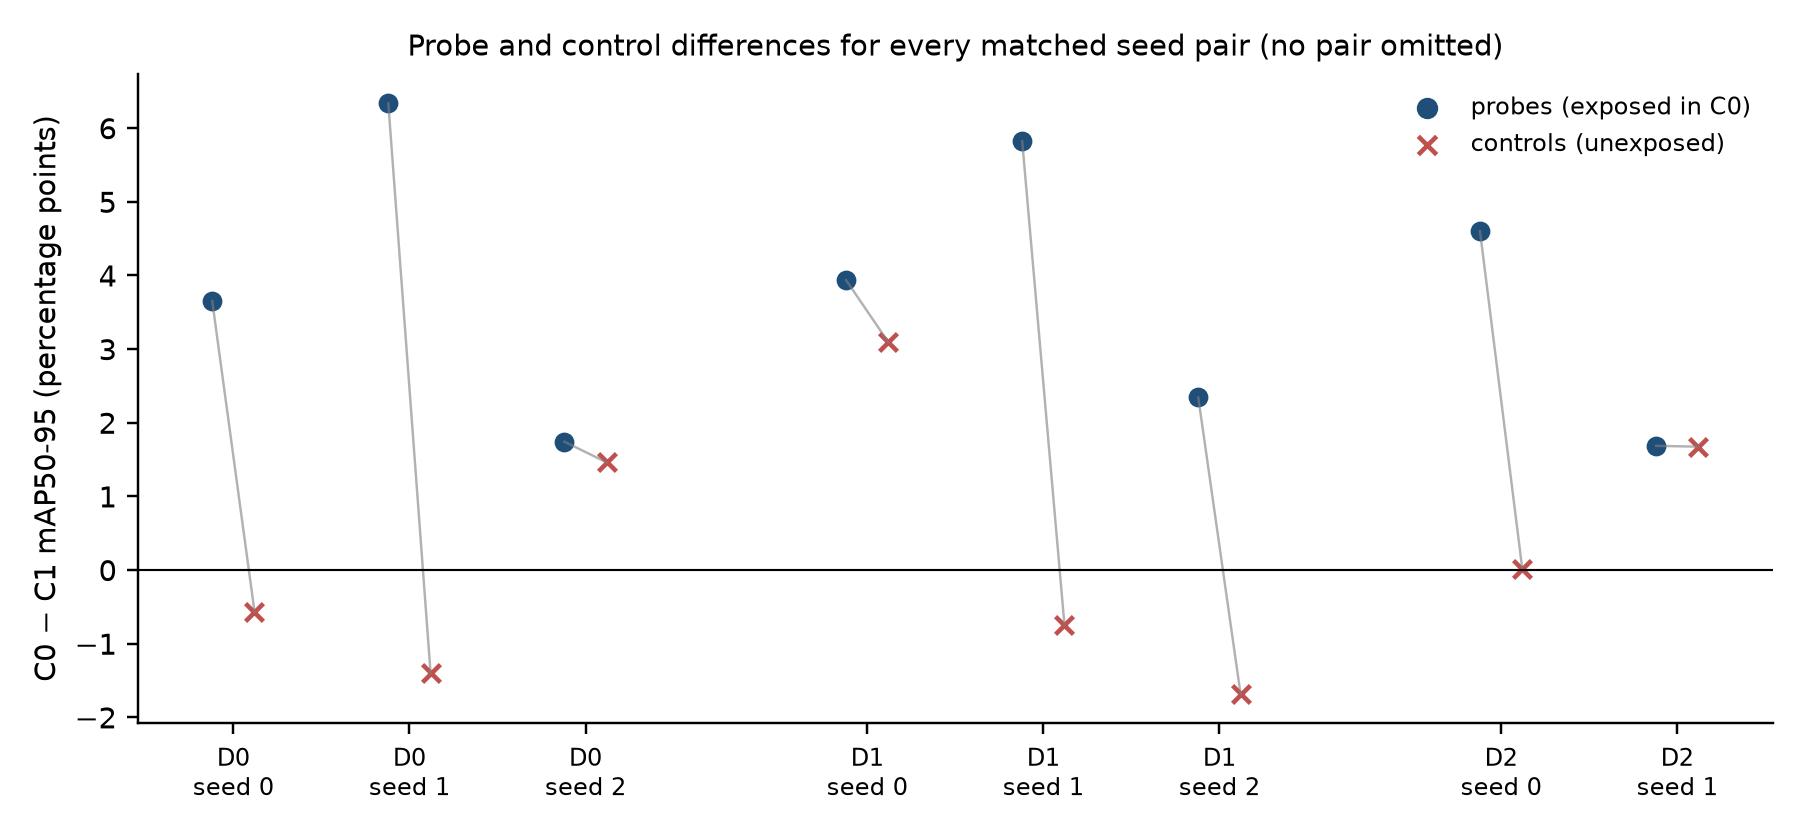
\includegraphics[width=0.9\linewidth]{figures/fig3_replication.png}\caption{Probe and control C0$-$C1 differences for every matched seed pair.}\label{fig:replication}\end{figure}
Table 1 lists every matched seed pair; none is omitted (see also Figure 1).

\begin{table}[htbp]\centering\small
\caption{C0 $-$ C1 mAP50-95 (percentage points) on fixed test sets.}
\begin{adjustbox}{max width=\linewidth}
\begin{tabular}{llllll}
\toprule
design & seed & overall & probes & controls & probes $-$ controls \\ \midrule
D0 & 0 & +1.75 & +3.65 & $-$0.56 & +4.22 \\
D0 & 1 & +2.36 & +6.34 & $-$1.40 & +7.73 \\
D0 & 2 & +1.16 & +1.74 & +1.46 & +0.28 \\
D1 & 0 & +3.70 & +3.94 & +3.09 & +0.84 \\
D1 & 1 & +2.91 & +5.82 & $-$0.75 & +6.57 \\
D1 & 2 & +0.20 & +2.34 & $-$1.68 & +4.02 \\
D2 & 0 & +2.69 & +4.60 & +0.02 & +4.58 \\
D2 & 1 & +1.65 & +1.69 & +1.68 & +0.01 \\
unweighted mean of 8 pairs &  & +2.05 & +3.77 & +0.23 & +3.53 \\
\bottomrule
\end{tabular}
\end{adjustbox}
\end{table}
\begin{table}[htbp]\centering\small
\caption{Design means and intervals (95\%). A: test sampling; B: training seeds; C: combined.}
\begin{adjustbox}{max width=\linewidth}
\begin{tabular}{lllllll}
\toprule
estimand & seeds & mean & A & B & C & P($\leq$0), C \\ \midrule
\textbf{D0 probes (primary)} & 3 & \textbf{+3.91} & +1.27, +6.77 & $-$1.82, +9.64 & \textbf{+0.41, +7.65} & 0.014 \\
D0 overall & 3 & +1.76 & +0.20, +3.76 & +0.27, +3.24 & $-$0.05, +3.95 & 0.030 \\
D0 probes $-$ controls & 3 & +4.08 & +0.79, +7.29 & $-$5.19, +13.34 & $-$0.97, +9.07 & 0.066 \\
D1 probes & 3 & +4.03 & +1.59, +6.92 & $-$0.29, +8.36 & +0.92, +7.51 & 0.006 \\
D1 probes $-$ controls & 3 & +3.81 & +0.84, +6.94 & $-$3.31, +10.94 & $-$0.65, +8.17 & 0.044 \\
D2 probes & 2 & +3.14 & +0.61, +5.93 & $-$15.37, +21.66 & $-$0.46, +6.51 & 0.045 \\
D2 probes $-$ controls & 2 & +2.30 & $-$0.87, +5.66 & $-$26.75, +31.34 & $-$2.42, +6.76 & 0.143 \\
pooled probes (3 designs) & 8 & +3.70 &  &  & +1.71, +5.70 &  \\
pooled probes $-$ controls & 8 & +3.37 &  &  & +0.68, +6.06 &  \\
pooled overall & 8 & +2.03 &  &  & +0.79, +3.27 &  \\
\bottomrule
\end{tabular}
\end{adjustbox}
\end{table}
\textbf{Primary endpoint.} The D0 probe effect was +3.91 points, with a combined interval of +0.41 to +7.65. The seed-only interval for three seeds includes zero.

\textbf{Selectivity.} The probe effect was positive in all eight seed pairs (minimum +1.69). Control differences scattered around zero (mean +0.23; range $-$1.68 to +3.09). The probe-minus-control contrast was positive in all eight pairs, but close to zero in two of them (+0.28 and +0.01). Within D0 alone its combined interval includes zero.

\textbf{Benchmark-level effect.} On the whole test set the effect was modest: +1.76 points in D0 and +2.03 pooled.

\subsection{Placebo analysis}
\begin{table}[htbp]\centering\small
\caption{Probe $-$ control contrast against 10,000 source-stratified random relabellings of test groups.}
\begin{adjustbox}{max width=\linewidth}
\begin{tabular}{llllll}
\toprule
design & seeds & observed & null mean (SD) & one-sided p & two-sided p \\ \midrule
D0 & 3 & +4.08 & +0.03 (1.82) & 0.013 & 0.024 \\
D1 & 3 & +3.81 & $-$0.02 (1.69) & 0.009 & 0.019 \\
D2 & 2 & +2.30 & +0.03 (1.62) & 0.078 & 0.154 \\
\bottomrule
\end{tabular}
\end{adjustbox}
\end{table}
In D0 and D1 the real probe set is atypical among same-sized group partitions of the test set. In D2 it is not clearly so.

\subsection{Exposure strength}
\begin{figure}[htbp]\centering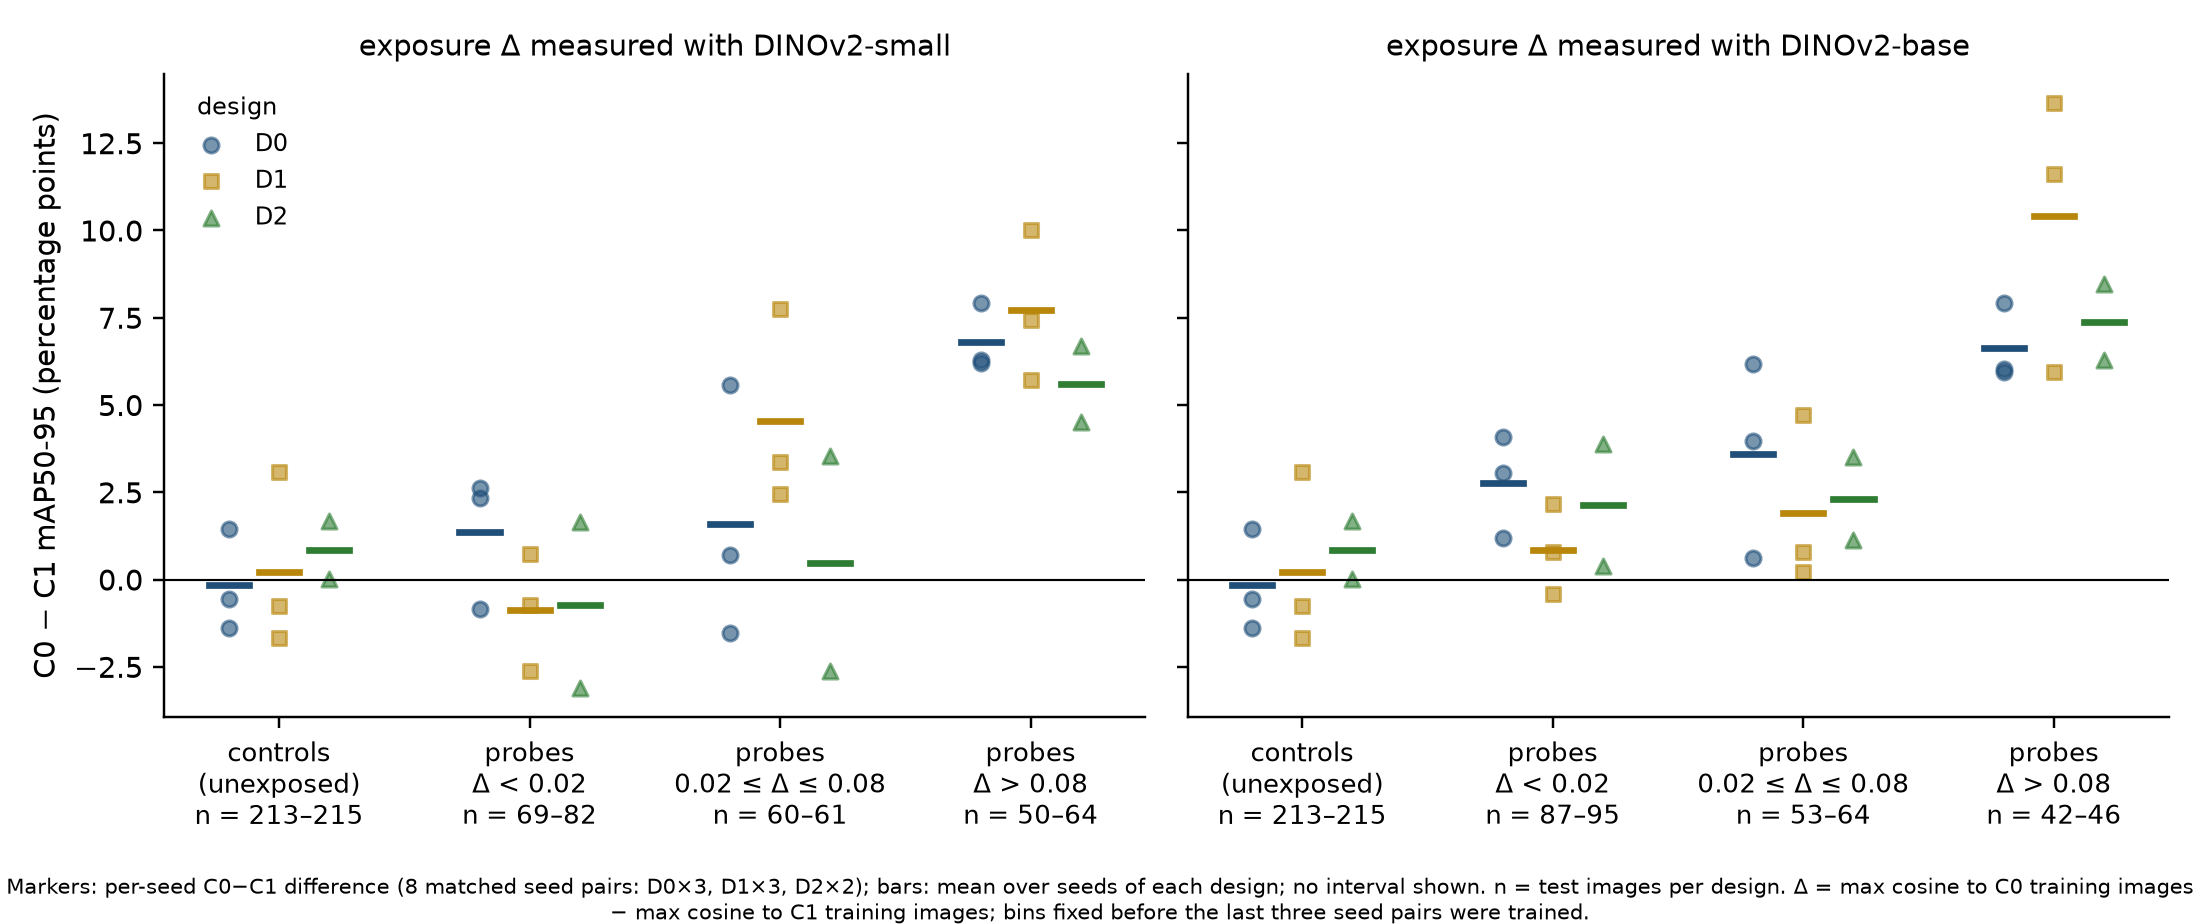
\includegraphics[width=\linewidth]{figures/fig1_exposure_gain.png}\caption{C0$-$C1 mAP50-95 by exposure stratum (left: DINOv2-small; right: DINOv2-base). Markers: per-seed differences (8 matched seed pairs); bars: design means; no interval drawn. n = test images per design.}\label{fig:exposure}\end{figure}
Figure 2 stratifies probes by exposure $\Delta$.

\textbf{Strongest stratum ($\Delta$ > 0.08; 50--64 images per design).} The mean difference was +6.85 points across the eight seed pairs (minimum +4.52). It exceeded the controls of the same design in every pair (mean excess +6.6). The three seed pairs trained after the strata were fixed followed the same pattern: +10.01 and +5.71 in D1, and +4.52 in D2.

\textbf{Weaker strata.} Probes with $\Delta$ < 0.02 differed by +0.00 on average, like controls. The middle stratum averaged +2.41.

\textbf{DINOv2-base.} With $\Delta$ measured by DINOv2-base, the strongest stratum averaged +6.64, +10.40 and +7.38 points in D0, D1 and D2.

\textbf{Continuous association.} The association between $\Delta$ and per-image recall gain was weak. Spearman $\rho$ was 0.15 (D0; 95\% CI 0.03--0.29), 0.12 (D1) and 0.08 (D2) with DINOv2-small, and 0.11--0.13 with DINOv2-base; only the first interval excludes zero.

\textbf{Reading.} The strongest pre-defined exposure stratum consistently showed the largest performance difference, while the continuous similarity--gain relationship was weak. We do not claim that gain increases smoothly with similarity.

\subsection{What the exposing images look like}
\begin{table}[htbp]\centering\small
\caption{AI-assisted visual adjudication of 60 D0 probe $\rightarrow$ nearest-exposing-mate pairs (coarse categories; not human-validated).}
\begin{adjustbox}{max width=\linewidth}
\begin{tabular}{ll}
\toprule
relationship & pairs \\ \midrule
near-exact duplicate & 0 \\
same specimen or capture series likely & 4 \\
same design / layout family & 9 \\
structurally related & 28 \\
not meaningfully related & 16 \\
ambiguous & 3 \\
\bottomrule
\end{tabular}
\end{adjustbox}
\end{table}
\textbf{What the pairs show.}

\begin{itemize}
\item \emph{No near-duplicates.} None of the 60 pairs was a near-exact duplicate, including the 20 pairs with DINOv2 cosine $\geq$ 0.934 (the ``near'' level).
\item \emph{Similarity tracks family, not identity.} DINO similarity was associated with visual relatedness ($\rho$ = 0.49), but at the level of design family rather than specimen identity.
\item \emph{Board-ID links.} Of 20 PCB-IND probes linked to their mates only by board-ID metadata, 14 had a nearest mate with no visible relationship, and 2 showed overlapping crops.
\item \emph{Earlier review.} In the earlier AI review of 300 similarity-audit candidates, none of 66 cross-source pairs was judged duplicate-like.
\end{itemize}
These observations motivate our terminology: we describe the manipulation as \textbf{train--test group exposure} to machine-detected visual-similarity groups, not as near-duplicate or same-board leakage.

\section{Replication and Sensitivity}
\textbf{D1: the control anomaly did not recur.} The first D1 seed showed a control gain of +3.09 points, almost as large as its probe gain. That pattern contradicts a purely exposure-specific effect, and it prompted two additional seeds. Their control differences were $-$0.75 and $-$1.68 (three-seed mean +0.22), while probe gains were +5.82 and +2.34. The original anomaly did not replicate. Training stochasticity is a plausible explanation, consistent with the 2.22-point control difference observed between two identically configured replicates, but it is not proven. With the other pre-existing C0 replicate for seed 1, the D1 seed-1 contrasts were probe +6.07, control +1.47 and probe $-$ control +4.60.

\textbf{D2: mixed replication.} D2 seed 0 resembled D0 (probes +4.60, controls +0.02). The probe-selective pattern weakened in the second D2 seed: probes and controls rose by the same amount (+1.69 and +1.68). D2's probe $-$ control interval includes zero and its placebo p-value is 0.08. We do not count D2 as a successful replication.

\textbf{Representation.} The strongest-exposure result held when $\Delta$ was measured with DINOv2-base (Section 7.3). The \emph{membership} of probes, however, depends on the embedding (Section 4).

\textbf{Pre-planned split by link type.} The analysis plan specified a split of probes by how they are linked to their mates: \emph{visually linked} (similarity pair, similarity component or crop sibling) versus \emph{metadata only} (same source board ID or design family, with no similarity link).

\begin{table}[htbp]\centering\small
\caption{C0 $-$ C1 mAP50-95 on probes, by link type (per-seed values).}
\begin{adjustbox}{max width=\linewidth}
\begin{tabular}{lllllll}
\toprule
design & visually linked: probes & per seed & mean & metadata only: probes & per seed & mean \\ \midrule
D0 & 111 & +2.75, +5.02, +1.69 & +3.15 & 83 & +15.57, +12.20, +6.16 & +11.31 \\
D1 & 116 & +4.88, +6.75, +3.04 & +4.89 & 77 & +6.57, +0.73, $-$0.14 & +2.39 \\
D2 & 116 & +3.89, +2.26 & +3.08 & 78 & +3.55, $-$2.73 & +0.41 \\
\bottomrule
\end{tabular}
\end{adjustbox}
\end{table}
\begin{itemize}
\item \emph{Visually linked probes:} positive in all eight seed pairs (+1.69 to +6.75).
\item \emph{Metadata-only probes:} a large gain in D0 that did not replicate in D1 or D2.
\end{itemize}
We therefore do not attribute the effect to shared board identity.

\section{Source-Held-Out Evaluation}
\begin{figure}[htbp]\centering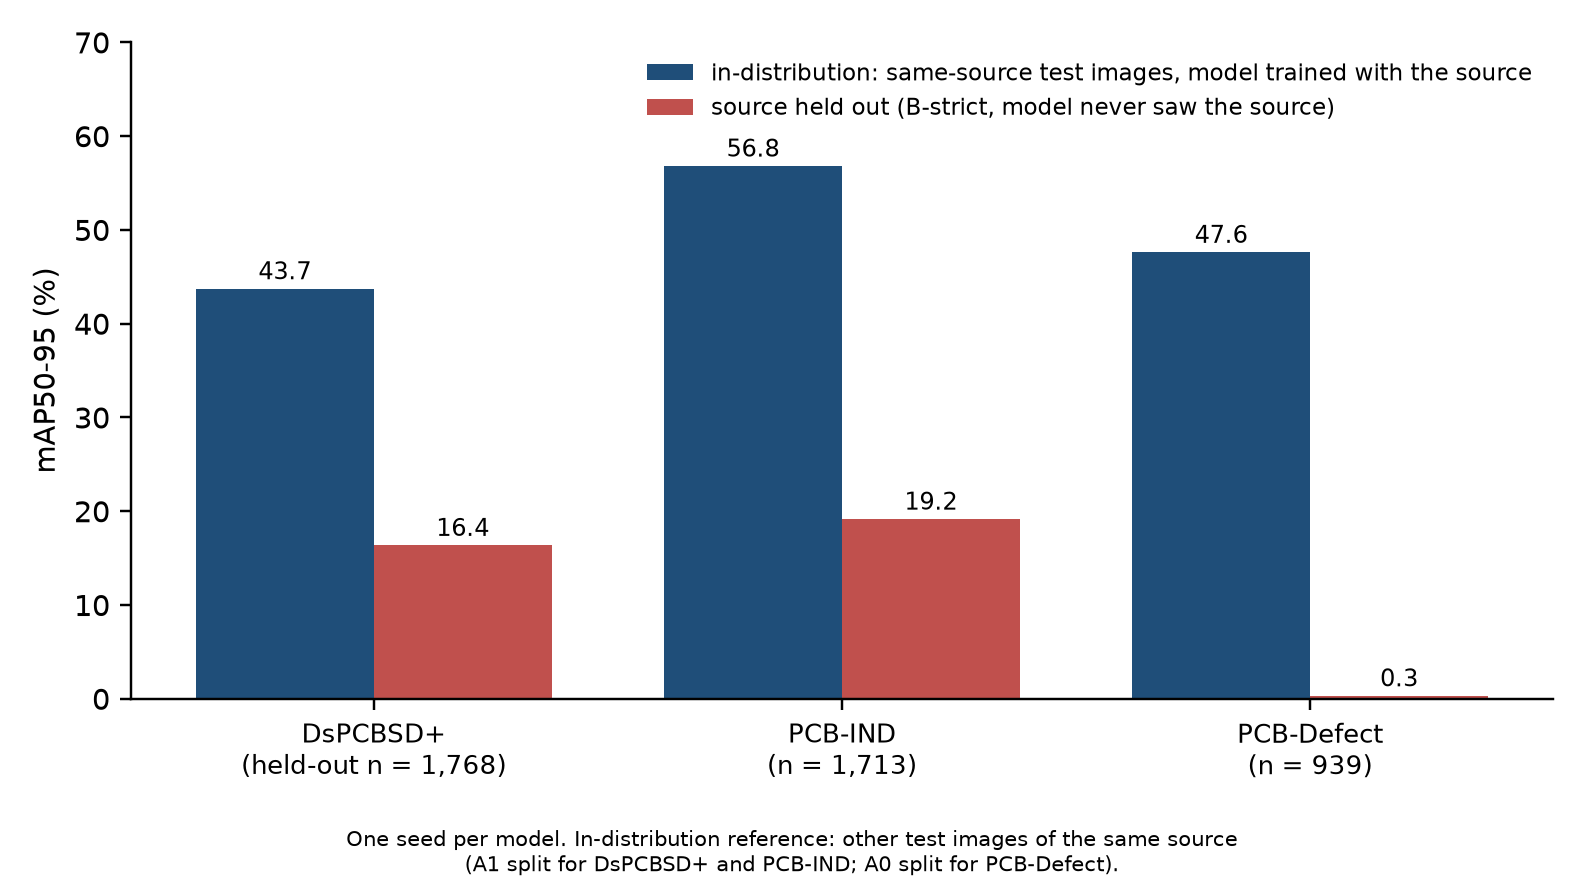
\includegraphics[width=0.8\linewidth]{figures/fig2_source_shift.png}\caption{In-distribution vs source-held-out mAP50-95 (one seed per model).}\label{fig:source}\end{figure}
\begin{table}[htbp]\centering\small
\caption{Source-held-out evaluation (mAP50-95, one seed per model).}
\begin{adjustbox}{max width=\linewidth}
\begin{tabular}{lllll}
\toprule
held-out source & held-out test images & in-distribution reference & source held out & difference \\ \midrule
DsPCBSD+ & 1,768 & 43.74 & 16.37 & $-$27.4 \\
PCB-IND & 1,713 & 56.82 & 19.17 & $-$37.7 \\
PCB-Defect & 939 & 47.62 & 0.33 & $-$47.3 \\
\bottomrule
\end{tabular}
\end{adjustbox}
\end{table}
The in-distribution reference uses other test images of the same source under a model trained on all sources (Figure 3).

\textbf{Keeping cross-source links.} A variant that keeps training images machine-linked to the held-out source did not help: DsPCBSD+ 15.21 and PCB-IND 19.72.

\textbf{PCB-Defect is not an evaluation error.} On the same 93 PCB-Defect test images, a model that saw the source scores 47.62 and localises 84 of 94 ground-truth boxes, all with the correct class. The held-out model behaves differently:

\begin{itemize}
\item it predicts confidently (median top confidence 0.70);
\item it assigns almost every prediction to spurious copper (2,373 of 2,378 at confidence $\geq$ 0.25);
\item it boxes ordinary copper traces and pads of the laboratory-fabricated boards;
\item it finds only 93 of 971 defects.
\end{itemize}
\textbf{Source identity.} Image width, height and file format alone identify the source with 100\% balanced accuracy (random forest, group-aware cross-validation).

These datasets encode strong acquisition and source signatures. Source-held-out evaluation therefore measures real domain shift, but not pure defect-semantic generalisation. The results do not show that the detector cannot learn the defect classes, nor that PCB-Defect is intrinsically harder.

\section{Limitations}
\begin{itemize}
\item \textbf{No independent human validation.} The relationships between grouped images were characterised only by AI-assisted visual adjudication from one model family. Fine-grained agreement was weak ($\kappa$ = 0.17).
\item \textbf{Machine-detected groups.} Groups come from embeddings, perceptual hashes and source metadata. Some links, especially cross-source and board-ID links, are not visually supported.
\item \textbf{Representation sensitivity.} Group membership changes substantially between DINOv2-small and DINOv2-base.
\item \textbf{Single architecture and domain.} Only YOLO11n on PCB defect crops was studied. Larger models or other domains may behave differently.
\item \textbf{Few seeds.} There are 2--3 seeds per design, so seed-only intervals are very wide. D0's probe-minus-control interval includes zero once seed variation is included.
\item \textbf{Training non-determinism.} Identically configured platform runs differ by 1--2 points on subsets.
\item \textbf{Mixed replication.} D2's second seed showed no probe-selective gain, and D1's first seed showed a control gain.
\item \textbf{Weak continuous trend.} The similarity--gain relationship is weak. The exposure strata were defined after the first five seed pairs were evaluated.
\item \textbf{Design imbalances.} Probes are grouped images and controls are mostly singletons. C0 has 4--6\% more training boxes than C1.
\item \textbf{Source confounding.} Source-held-out results confound acquisition, substrate, resolution and crop generation.
\item \textbf{No deployment data.} All test images are public-dataset crops; nothing here estimates production-line performance.
\end{itemize}
\section{Discussion}
\textbf{What the effect is.} In this benchmark, training on a test image's machine-detected group-mates was associated with about 3.7 additional mAP50-95 points on that image, while unexposed images changed little on average. The gain was carried mostly by the most strongly exposed images. Their exposing training images are, by AI adjudication, mostly same-design or structurally related, not copies. ``Familiarity with a board family, layout or capture condition'' therefore describes the observations better than ``memorisation of duplicates''. Confirming that interpretation requires human review.

\textbf{How much it matters.} Across a whole test set the optimism was about two points. This is of the same order as the variation between identically configured training runs, and as the margins by which detector variants are often compared on PCB benchmarks. Benchmarks that report improvements of a few points on randomly split PCB data should use group-aware splits and replicate training runs.

\textbf{What matters more.} A detector trained on two sources lost 27--47 points on a third. For practitioners, evaluating on a held-out line, imaging setup or board family is a more important safeguard than deduplication. Because source identity is trivially encoded in image metadata, such evaluations should be interpreted as acquisition-shift tests.

\textbf{Negative results.} We report the D1 control anomaly, the weakened D2 seed and the weak continuous trend in the main text because they bound the claims. The probe-selective effect is consistent across designs on average, but not in every training run.

\section{Conclusion}
In a controlled PCB detection benchmark, train--test group exposure produced a real but modest optimism. It was concentrated among the most strongly exposed test images, it replicated imperfectly across independently drawn designs, and it was an order of magnitude smaller than the cost of an unseen acquisition source. Group-aware splits and replicated training runs are good benchmark hygiene. Source-held-out evaluation is the more consequential safeguard. Independent human review of the grouped image pairs remains outstanding.

\section{Data and code availability}
\textbf{Code.} Code, manifests, configuration, checkpoint hashes, per-image evaluation outputs and analysis scripts are available at https://github.com/canblmz1/openinspect-trust (Apache-2.0). The source datasets are available from their publishers under CC BY 4.0~\cite{lv2024dspcbsd,yan2026pcbind,rashid2025pcbdefect}; the release lists every change made to them.

\textbf{Model weights.} Model weights are not redistributed. Each checkpoint is identified by its SHA-256 hash, and every model can be retrained from the published configuration, seeds and split manifests. Retrained results will differ within the run-to-run variation reported above.


\bibliographystyle{plain}
\bibliography{references}
\end{document}
